\documentclass{beamer}
%
% Choose how your presentation looks.
%
% For more themes, color themes and font themes, see:
% http://deic.uab.es/~iblanes/beamer_gallery/index_by_theme.html
%
\mode<presentation>
{
  \usetheme{NYU}      % or try Darmstadt, Madrid, Warsaw, ...
  \usecolortheme{default} % or try albatross, beaver, crane, ...
  \usefonttheme{default}  % or try serif, structurebold, ...
  \setbeamertemplate{navigation symbols}{}
  \setbeamertemplate{caption}[numbered]
} 

\usepackage[english]{babel}
\usepackage[T1]{fontenc}
\usepackage[utf8x]{inputenc}
\usepackage{hyperref}

\begin{document}


\title[CONTROL SYSTEMS]{EE18BTECH11043}
\subtitle{ASSINGMENT}
\author{THOTAMALLA YUVATEJA}
\institute{IIT HYDERABAD}
\date{\today}
\titlegraphic{\hfill
\includegraphics[height=1.5cm]{nyu_shanghai}}
\begin{frame}
  \titlepage
\end{frame}
\begin{center}
\\{This document is generated by \LaTeX}
 \end{center}
\\{Question 4}
\\{When a unit ramp input is applied to the unity feedback system having closed loop transfer function $$
    \frac{C(s)}{R(s)} = \frac{Ks + b}{s^2 + as + b}$ (a$>$,b$>0$,K$>$0),the steady state error will be 
\\
\\
\\A.0  
\\
\\B.$\frac{a}{b}$ 
\\
\\C.$\frac{a+K}{b}$
\\
\\D.$\frac{a-K}{b}$
 }
\item \textbf{solution}
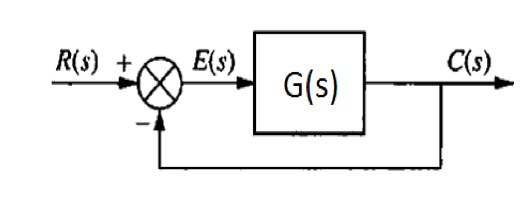
\includegraphics[width=.6\textwidth]{gvvpic (2).png}
\begin{equation}
    T(S) = \frac{C(S)}{R(S)}
\end{equation}
    
\begin{equation}
    C(t) = r(t) - \tau(t)
\end{equation}

\\Apply L.T to above equations 
\\
\\$E(s)=R(s)[1 - T(s)]$
\\
\\Steady state error is a property of the input/output response for a linear system. In a good control system, steady-state error should be minimum.
\\


\\$e_{ss}$ = C(\infty) = $$\lim_{s\to\ 0} s\times\dfrac{1}{s^2}\times[1-\dfrac{[Ks+b]}{s^2+as+b}]$$
\\
\\
\\ \implies$$\lim_{s\to\ 0} \dfrac{1}{s}\times[\dfrac{s^2+s[a-K]}{s^2+as+b}]$$
\\
\\
\\ \implies$$\lim_{s\to\ 0}\dfrac{s+(a-K)}{s^2+as+b}$$
\\
\\
\\ \implies $e_{ss}=\dfrac{a-K}{b}$
\\

\\
\\ We can find steady state error using the final value theorem as shown above
\\
\\E(s) is the Laplace transform of the error signal, e(t)
\\
\\The output of the summing point is our equation 3
\\
\\Substitute C(s) value in the above equation.
\\
\\Substitute E(s)value in the steady state error formula
\\
\\By finding that limit value we get our steady state error value 






\end{document}
